\clearpage
\section{Contribution}
\label{contribution}

In \S\ref{dtw}, the dynamic time warping distance was presented as a 
FOM for measuring the similarity between time series, whether they 
were model-to-simulator comparisons or model-to-model comparisons.
The distances alone, though, have the inverse meaning when trying to 
compute a FOM for contribution to a fuel cycle.  For example, the 
question may be posed as, ``Do LWRs or FRs impact the total power generated 
more over the entire fuel cycle time domain?'' 
While distances can answer this question, smaller 
disantances have higher impact. Preferably, a higher FOM score would yield a 
higher impact. Furthermore, the distances in the previous section have
the same units as the cost matrix and are similarly bounded. A better 
FOM for contribution would be unitless and defined on the range $[0,1]$.

Thus, let $c$ be the \emph{contribution} FOM that satisfies the above 
constraints. To define $c$, first define $D$ as the maximal possible 
distance from the model of the total. Recall that this time series has length $A$.
$D$ is, therefore, the L1 norm of the model of the total time series divided
by twice its length. 
\begin{equation}
\label{D-def}
D(m_*^\Total) = \frac{\left|m_*^\Total\right|_1}{2A}
\end{equation}
This is the equivalent to computing the DTW distance
between $m_*^\Total$ and the curve where the metric is zero for all time 
(i.e. the t-axis itself).  This relies on the notion that 
metric is necessarily non-negative everywhere.  If the metric is allowed to 
be negative, another baseline curve could be chosen. $D$ would then be 
computed as the DTW distance between the total model and this baseline.
However, in most cases the metrics are not allowed to be negative, 
a baseline of zero is suitable, and Equation \ref{D-def} applies.

The contribution figure-of-merit of a given partition to the total is thus 
defined as follows:
\begin{equation}
\label{cont}
c^i = 1 - \frac{d(m_*^\Total, m_*^i)}{D(m_*^\Total)}
\end{equation}
$D$ is seen to normalize the model-to-model distance while subtracting this
ratio from unity makes higher contribution values more important.  
Using the sample data, $c^\LWR = 0.298$ and $c^\FR = 0.859$. This again shows
that the FRs are more important to the total power of the whole cycle.
Here though, higher contribution scores yield higher importance and the values
are always between zero and one.

Note that even though $c$ is a fraction, it is not normalized across 
partitions. Namely, the sum of all contributions for all $I$ partitions
is on the following range, which is not $[0, 1]$:
\begin{equation}
\label{sum-c-range}
0 \le \sum_i^I c^i \le I
\end{equation}
It is easy to imagine an alternative FOM that divides $c^i$ by $I$. However, 
this was not done here because the choice of $I$ (the number of partitions)
can be made arbitrarily large.  In the sample calculations $I=2$ for LWRs and
FRs.  However, $I$ could have been set to 3 by including small modular reactor
(SMRs) which have not yet been built and produce no power.  $I$ could then be 
increased to 4 or higher by including more non-existent reactor types.

Dividing the contribution by $I$ is not sufficient to 
normalize the sum of the $c^i$, in general, because the 
contribution is inherently a cumulative measure. If a component ever had a 
non-zero value, it will always be seen to have contributed something. 
Because of this constraint on the total, $\sum c^i$ can never
reach $I$ unless there is only a single component or the 
total is zero valued everywhere (which implies that the constituents are also 
zero). Thus, dividing $c^i$ by $I$ with the aim of normalizing the 
sum of the $c^i$ is incorrect for any situation of interest to a fuel 
cycle benchmark.

If a truly normalized version of contribution is desired, it must 
use the sum of the actual contributions. Define the normalized contribution 
as $|c^i|$, 
\begin{equation}
\label{norm-ci}
\left|c^i\right| = \frac{c^i}{\sum_j^I c^j}
\end{equation}
The disadvantage with the normalized contribution is that all of the 
individual component $c^i$ must be known prior to the normalization. 
Furthermore, since the sum is typically greater than 1, the difference 
between components is often smaller in the normalized form than in the
more pronounced unnormalized contribution.
The only advantages that $|c^i|$ confers over $c^i$ are that it is defined on 
the range $[0,1]$ and that $\sum |c^i| = 1$. Otherwise, both versions of the FOM
have the same properties with respect to having a zero baseline, the 
interpretation that higher values are higher impact to the total, and that they 
are non-judgmentally derived from models rather than simulators.

\begin{figure}[htb]
\centering
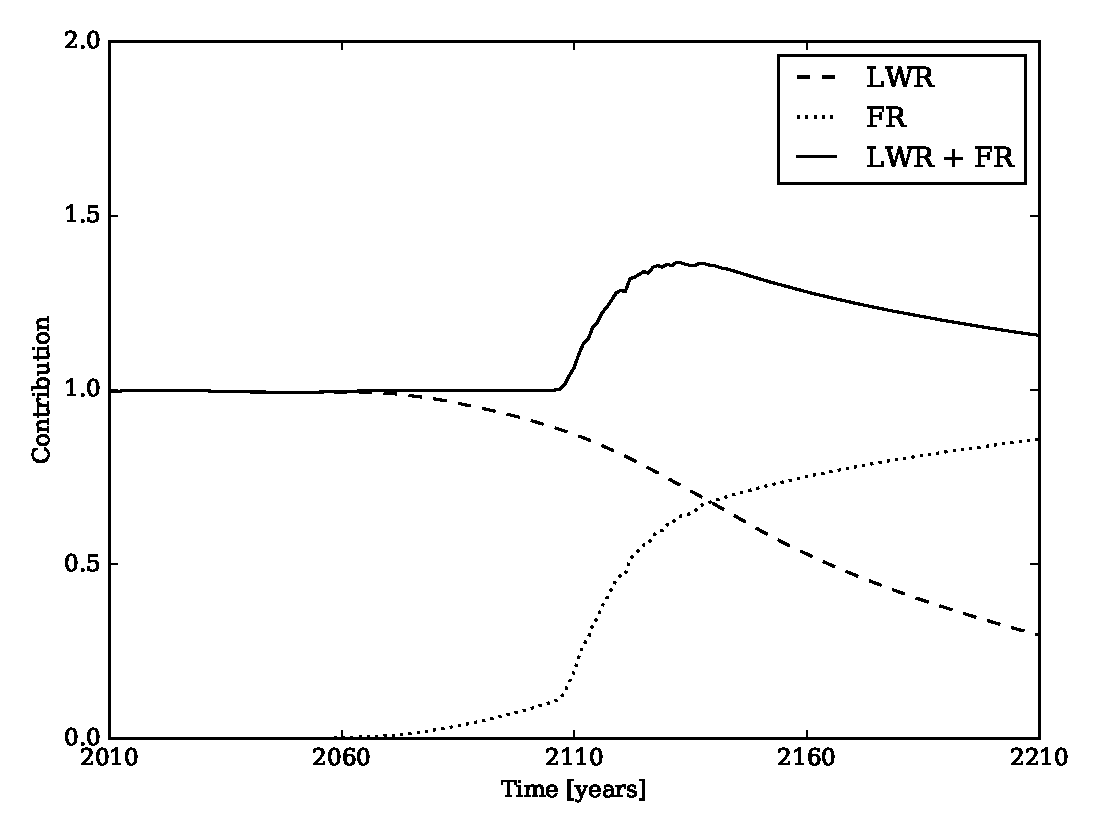
\includegraphics[width=0.9\textwidth]{c-of-t.eps}
\caption{Contribution of LWRs and FRs to total generated power as a 
function of time.}
\label{c-of-t}
\end{figure}

\begin{figure}[htb]
\centering
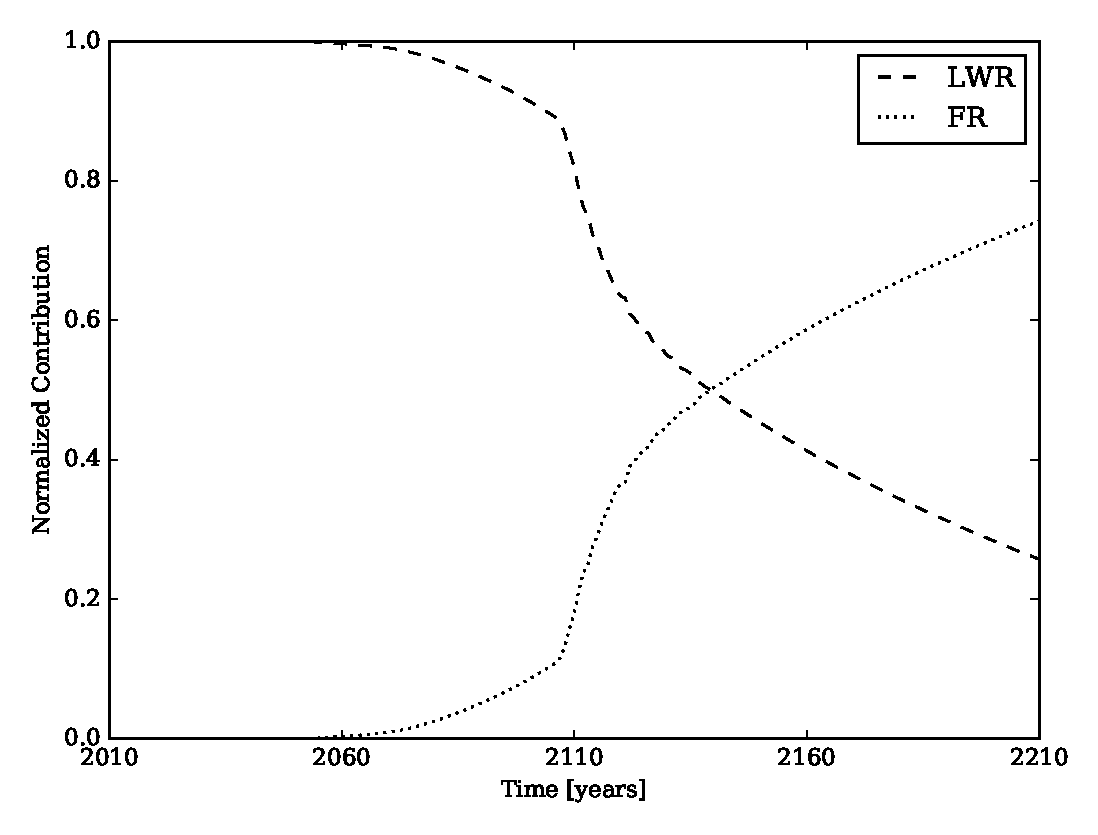
\includegraphics[width=0.9\textwidth]{normc-of-t.eps}
\caption{Normalized contribution of LWRs and FRs to total generated power 
as a function of time.}
\label{normc-of-t}
\end{figure}

Both $c^i$ and $|c^i|$ can be viewed as a function of time.
Doing so in a nuclear fuel cycle benchmark may help identify artifacts in the
calculation that are the result of the time domain chosen for the benchmark itself.
For instance, the FR contribution is expected to overtake the LWR contribution
and this does not occur or occurs very close to the maximum simulation time, 
this implies that the time horizon of the benchmark should be increased.
Figures \ref{c-of-t} \& \ref{normc-of-t} display the contribution and 
normalized contribution respectively for both LWRs and FRs over the full 
time domain. From these figures, the point where FRs become more important 
than LWRs is seen to be approximately year 2140.

It is worth noting that for all metrics for which the above contribution FOMs
are computable, direct integration of the Gaussian process models over 
the whole time domain can also provide a FOM. This is because 
contribution requirement that the metric have a linearly combined total 
implies that the metric is also integrable. A direct integration
FOM would thus share the property that higher values indicate higher impact
to the total. However, the contribution FOMs may still be desirable over 
integration-based FOMs.  This is because the DTW cost compounds the 
differences in the time series. As a result, the DTW distance based 
contributions are relatively more distinct than a model integration 
contribution. This extra emphasis on diverging contribution values may be 
desirable as the purpose of a FOM is to highlight differences. 
